%%%%%%%%%%%%%%%%%%%%%%%%%%%%%%%%%%%%%%%%%
% Beamer Presentation
% LaTeX Template
% Version 1.0 (10/11/12)
%
% This template has been downloaded from:
% http://www.LaTeXTemplates.com
%
% License:
% CC BY-NC-SA 3.0 (http://creativecommons.org/licenses/by-nc-sa/3.0/)
%
%%%%%%%%%%%%%%%%%%%%%%%%%%%%%%%%%%%%%%%%%

%----------------------------------------------------------------------------------------
%	PACKAGES AND THEMES
%----------------------------------------------------------------------------------------

\documentclass{beamer}

\mode<presentation> {

% The Beamer class comes with a number of default slide themes
% which change the colors and layouts of slides. Below this is a list
% of all the themes, uncomment each in turn to see what they look like.

%\usetheme{default}
%\usetheme{AnnArbor}
%\usetheme{Antibes}
%\usetheme{Bergen}
%\usetheme{Berkeley}
%\usetheme{Berlin}
%\usetheme{Boadilla}
%\usetheme{CambridgeUS}
%\usetheme{Copenhagen}
%\usetheme{Darmstadt}
%\usetheme{Dresden}
%\usetheme{Frankfurt}
%\usetheme{Goettingen}
%\usetheme{Hannover}
%\usetheme{Ilmenau}
%\usetheme{JuanLesPins}
%\usetheme{Luebeck}
\usetheme{Madrid}
%\usetheme{Malmoe}
%\usetheme{Marburg}
%\usetheme{Montpellier}
%\usetheme{PaloAlto}
%\usetheme{Pittsburgh}
%\usetheme{Rochester}
%\usetheme{Singapore}
%\usetheme{Szeged}
%\usetheme{Warsaw}

% As well as themes, the Beamer class has a number of color themes
% for any slide theme. Uncomment each of these in turn to see how it
% changes the colors of your current slide theme.

%\usecolortheme{albatross}
%\usecolortheme{beaver}
%\usecolortheme{beetle}
%\usecolortheme{crane}
%\usecolortheme{dolphin}
%\usecolortheme{dove}
%\usecolortheme{fly}
%\usecolortheme{lily}
%\usecolortheme{orchid}
%\usecolortheme{rose}
%\usecolortheme{seagull}
%\usecolortheme{seahorse}
%\usecolortheme{whale}
%\usecolortheme{wolverine}

%\setbeamertemplate{footline} % To remove the footer line in all slides uncomment this line
%\setbeamertemplate{footline}[page number] % To replace the footer line in all slides with a simple slide count uncomment this line

%\setbeamertemplate{navigation symbols}{} % To remove the navigation symbols from the bottom of all slides uncomment this line
}

\usepackage{graphicx} % Allows including images
\usepackage{booktabs} % Allows the use of \toprule, \midrule and \bottomrule in tables
\usepackage{subfig}
\usepackage{multicol}
\usepackage{stfloats}
\usepackage{hyperref}
\usepackage{multicol}
\usepackage[flushleft]{threeparttable}
\usepackage{mathtools}
\usepackage{csquotes}
\newenvironment{conditions}
{\par\vspace{\abovedisplayskip}\noindent\begin{tabular}{>{$}l<{$} @{${}={}$} l}}
	{\end{tabular}\par\vspace{\belowdisplayskip}}
\DeclarePairedDelimiter\ceil{\lceil}{\rceil}
\DeclarePairedDelimiter\floor{\lfloor}{\rfloor}
%----------------------------------------------------------------------------------------
%	TITLE PAGE
%----------------------------------------------------------------------------------------

\title[FPGA Security]{Automated Detection and Analysis of Hardware Trojans in FPGAs} % The short title appears at the bottom of every slide, the full title is only on the title page

\author{Nicholas Houghton} % Your name
\institute[UVIC] % Your institution as it will appear on the bottom of every slide, may be shorthand to save space
{
University of Victoria \\ % Your institution for the title page
\medskip
\textit{nhoughto@uvic.ca} % Your email address
}
\date{\today} % Date, can be changed to a custom date

\begin{document}

\begin{frame}
\titlepage % Print the title page as the first slide
\end{frame}

\begin{frame}
\frametitle{Overview} % Table of contents slide, comment this block out to remove it
\tableofcontents % Throughout your presentation, if you choose to use \section{} and \subsection{} commands, these will automatically be printed on this slide as an overview of your presentation
\end{frame}

%----------------------------------------------------------------------------------------
%	PRESENTATION SLIDES
%----------------------------------------------------------------------------------------

\section{Introduction}
\begin{frame}
	\frametitle{Introduction: Background}
	\begin{itemize}
		\item What are hardware trojans?
		\item How are devices affected by them?
		\item How do they work?
	\end{itemize}
\end{frame}

\begin{frame}
	\frametitle{Introduction: Objectives}
	\begin{enumerate}
		\item Devise a method to detect trojans in FPGAs
		\item Devise a method to describe descovered trojans
		\item Build an application to automate these processes.
		\item Automate the visualization technique presented in~\cite{samerAttribute}
	\end{enumerate}
\end{frame}

\begin{frame}
	\frametitle{Introduction: Two New Applications}
	\begin{itemize}
		\item Automated Hardware Trojan Detector (desktop application)
		\item The Hardware trojan system (website)
	\end{itemize}
\end{frame}

%%%%%%%%%%%%%%%%%%%%%%%%%%%%%%%%%%%%%%%%%%%
\section{Trojan Detector}
\begin{frame}
	\frametitle{Trojan Detector: Use-Case}
	\begin{figure}
		\centering
		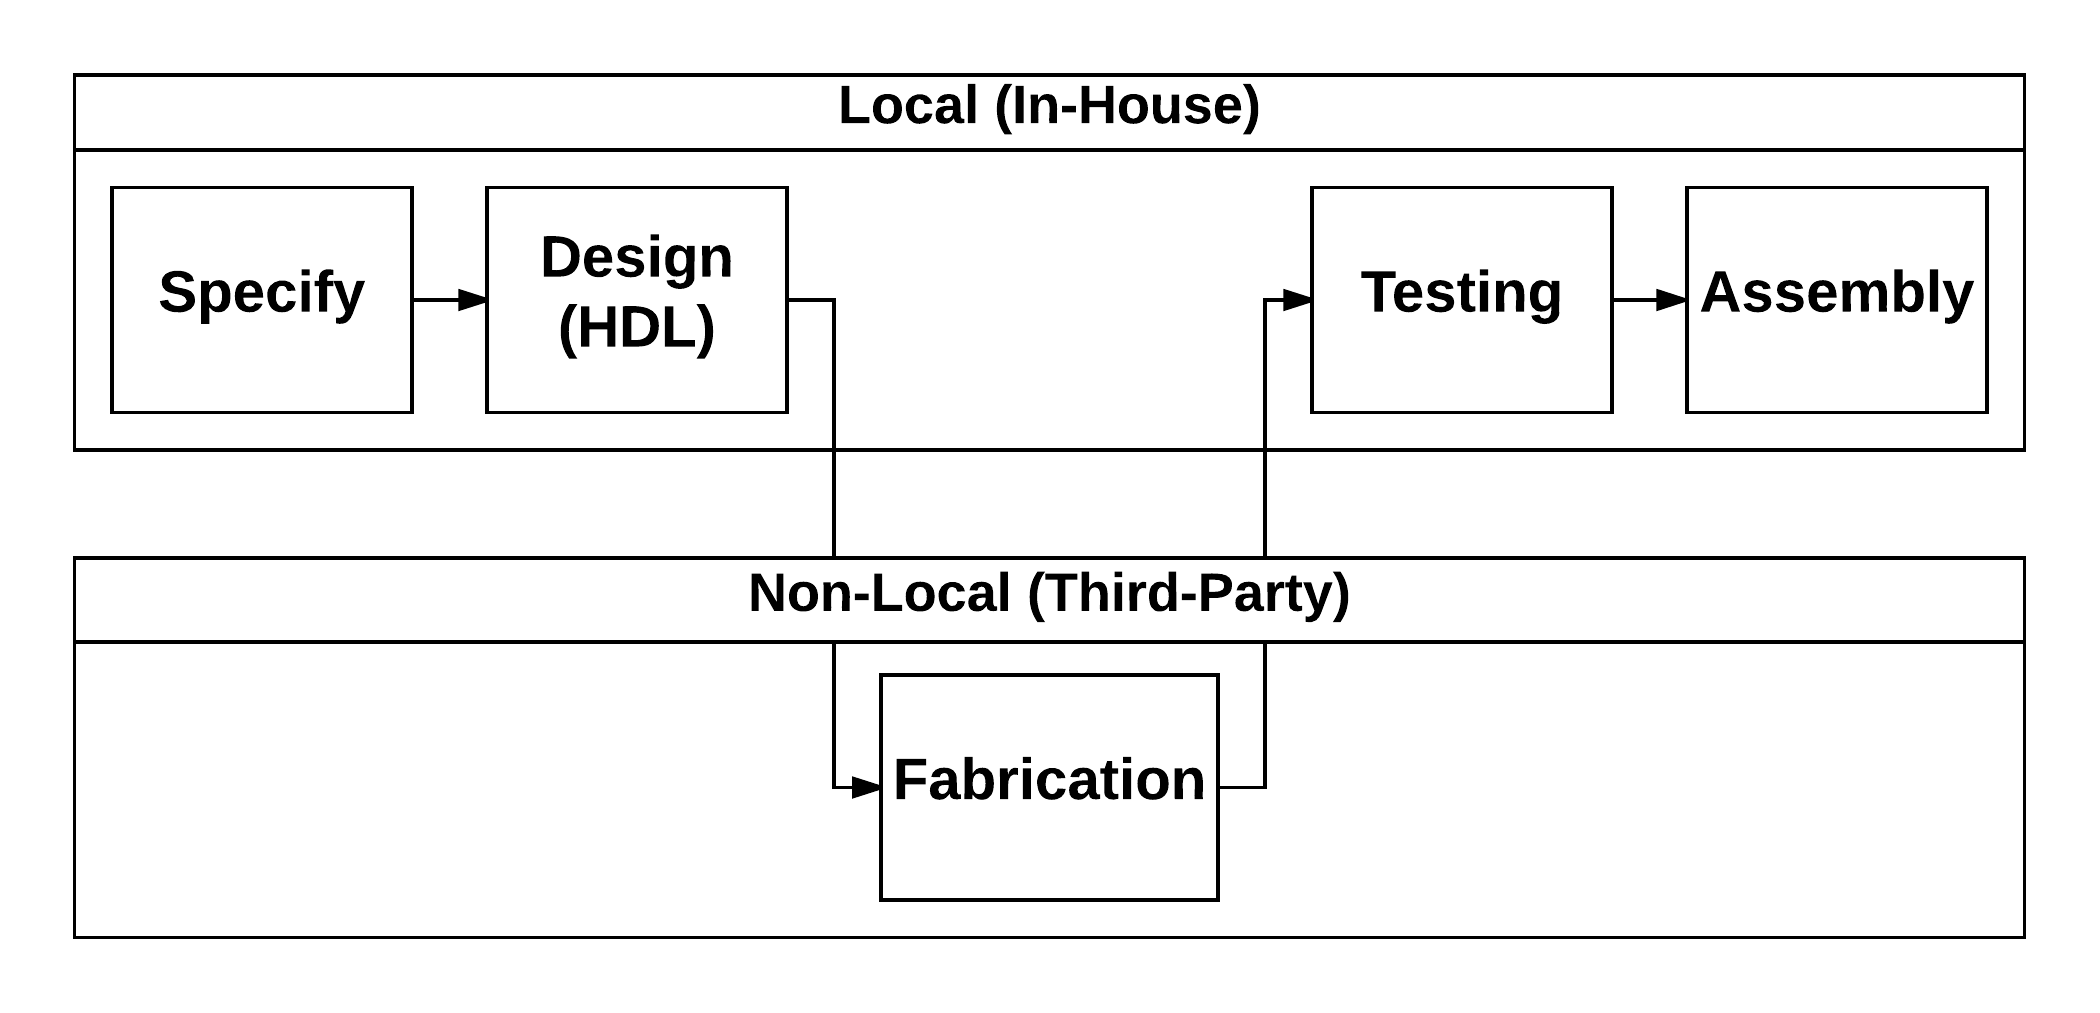
\includegraphics[width=0.7\linewidth]{../NewAutomated_V4/Figures/Concept}
		\caption[Use-Case]{Use-Case}
		\label{fig:Concept}
	\end{figure}
\end{frame}

\begin{frame}
	\frametitle{Trojan Detector: Methodology}
	\begin{figure}
		\centering
		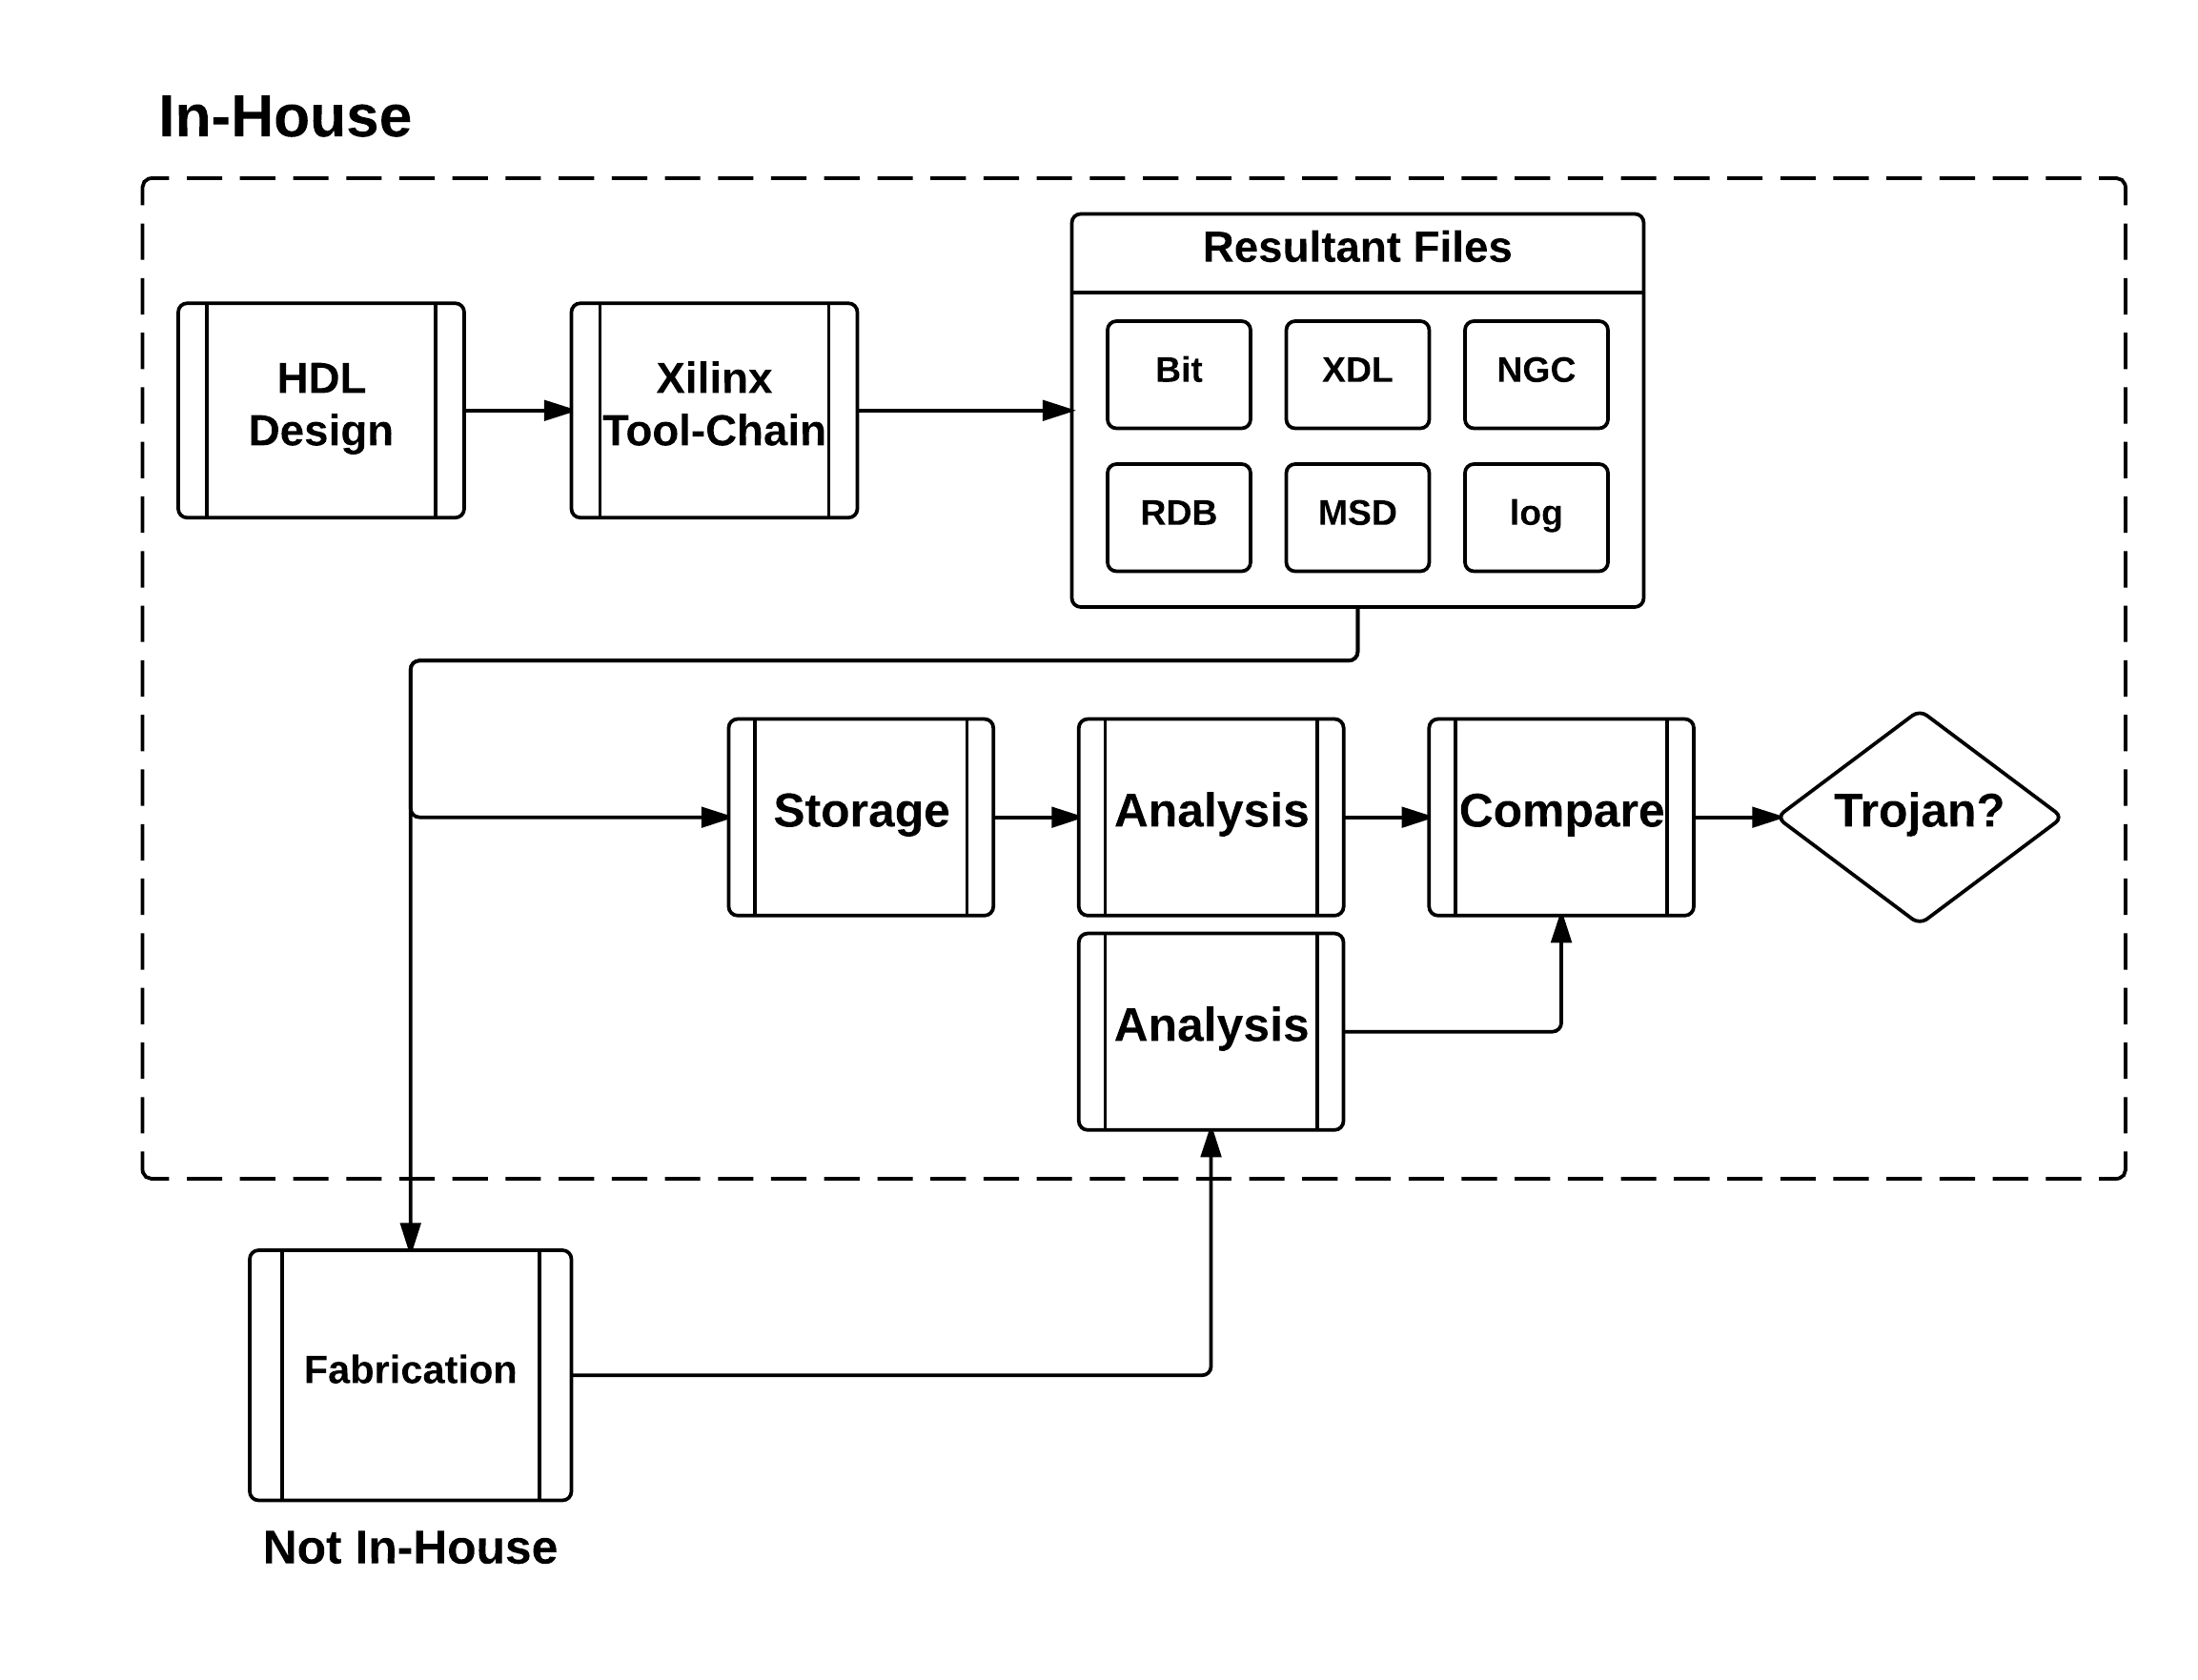
\includegraphics[width=0.7\linewidth]{../Thesis/Figures/methodologyOverview}
		\caption[Methdology Overview]{Methdology Overview}
		\label{fig:methodologyOverview}
	\end{figure}
\end{frame}

\begin{frame}
	\frametitle{Trojan Detector: FPGA}
	FPGA: Field Programmable Gate-Array
	\begin{figure}
		\centering
		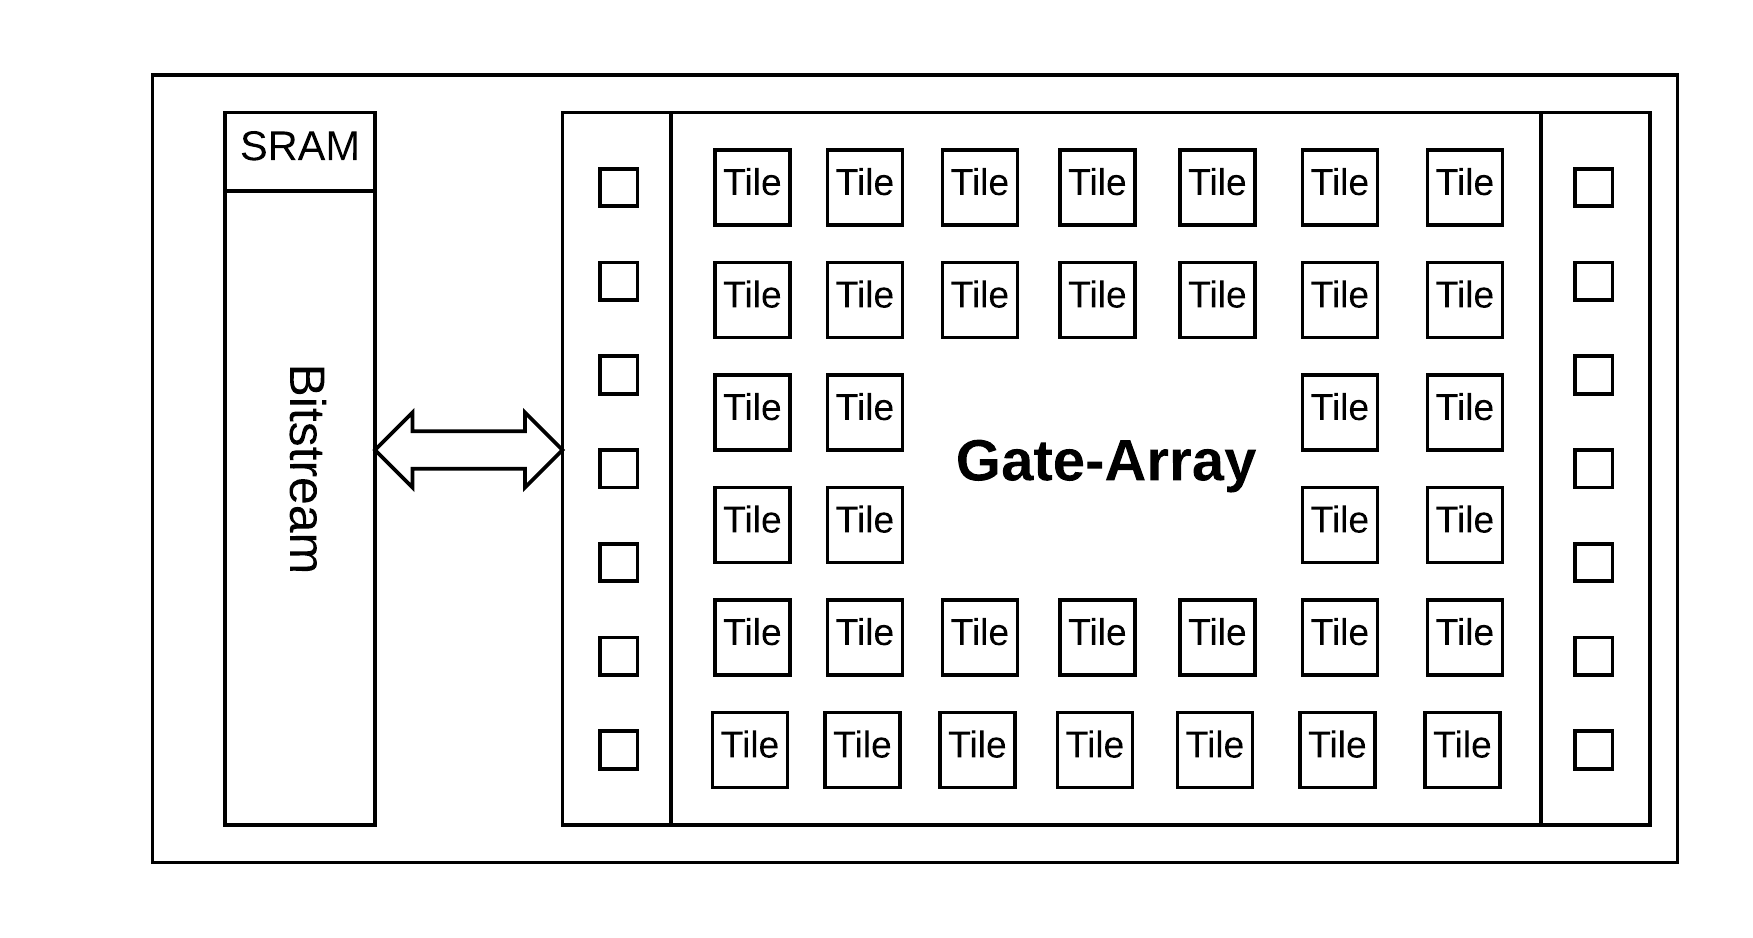
\includegraphics[width=0.7\linewidth]{../Thesis/Figures/architecture}
		\caption[Simplified FPGA Layout]{Simplified FPGA Layout}
		\label{fig:architecture}
	\end{figure}
\end{frame}

\begin{frame}
	\frametitle{Trojan Detector: Gate-Array Architecture}
	\begin{figure}
		\centering
		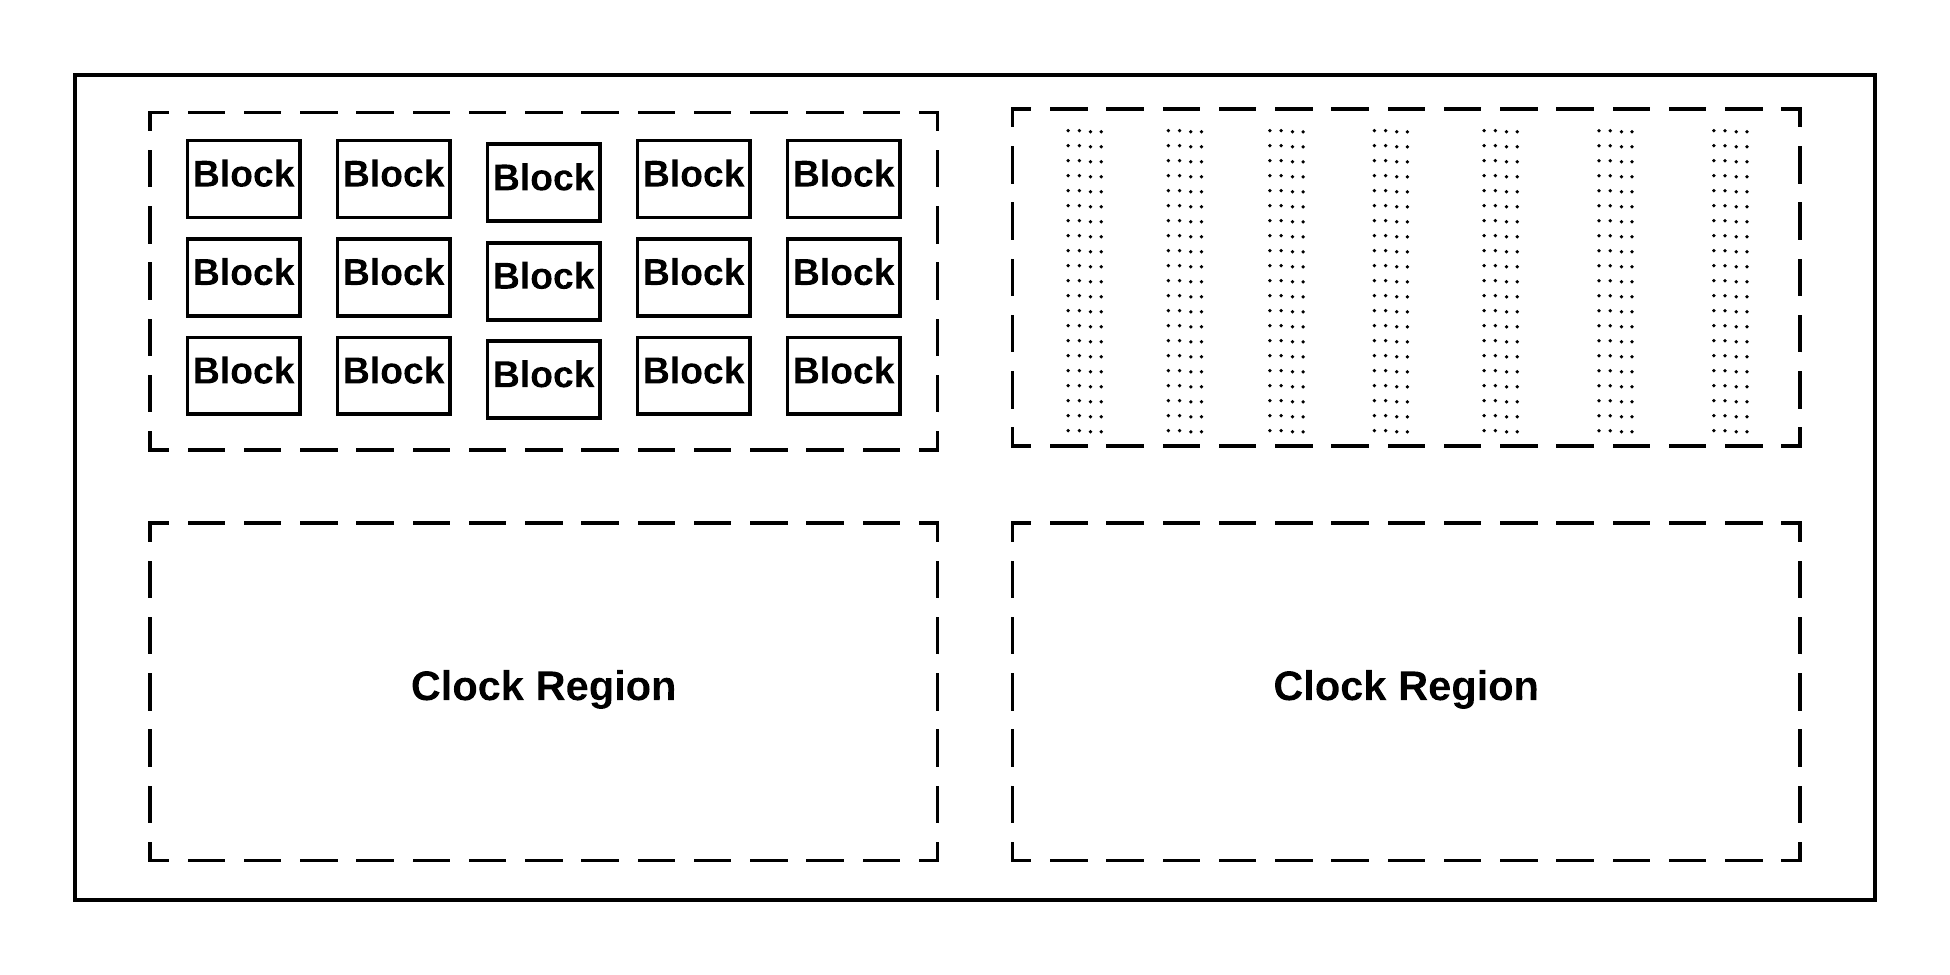
\includegraphics[width=0.7\linewidth]{../Thesis/Figures/FPGA}
		\caption[Gate-Array of Block Columns]{Gate-Array of Block Columns}
		\label{fig:FPGA}
	\end{figure}
\end{frame}

\begin{frame}
	\frametitle{Trojan Detector: Sub Columns}
	\begin{figure}
		\centering
		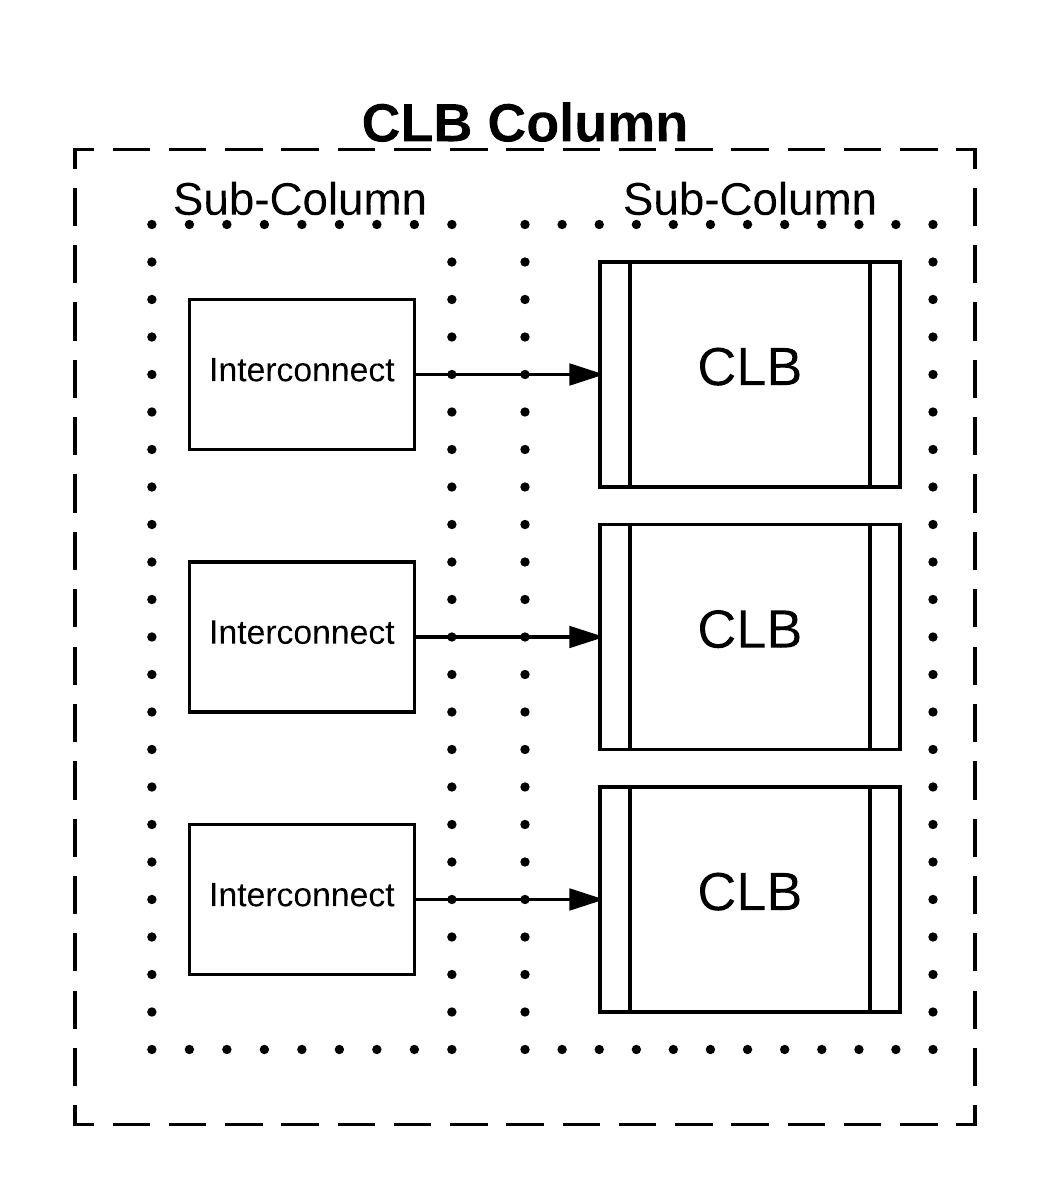
\includegraphics[width=0.5\linewidth]{../Thesis/Figures/column}
		\caption[Column Composition]{Column Composition}
		\label{fig:column}
	\end{figure}
\end{frame}

\begin{frame}
	\frametitle{Trojan Detector: Frame Addressing}
	\begin{table}
		\centering
		\caption{Bitstream Frame Address Structure}
		\label{tbl:frameAddress}
		\resizebox{\textwidth}{!}{
			\begin{tabular}{|c|c|c|c|c|c|c|c|c|c|c|c|c|c|c|c|c|c|c|c|c|c|c|c|c|c|c|c|c|c|c|c|}
				\hline
				\multicolumn{8}{|c|}{Unused} & \multicolumn{3}{c|}{BA} & T & \multicolumn{5}{c|}{Row Address} & \multicolumn{8}{c|}{Major Address} & \multicolumn{7}{c|}{Minor Address} \\ \hline
				31 & 30 & 29 & 28 & 27 & 26 & 25 & 24 & 23 & 22 & 21 & 20 & 19 & 18 & 17 & 16 & 15 & 14 & 13 & 12 & 11 & 10 & 9 & 8 & 7 & 6 & 5 & 4 & 3 & 2 & 1 & 0 \\ \hline
				0 & 0 & 0 & 0 & 0 & x & x & x & x & x & x & x & x & x & x & x & x & x & x & x & x & x & x & 0 & 0 & 0 & 0 & 0 & 0 & 0 & 0 & 0 \\ \hline
			\end{tabular}		
		}
	\end{table}
\end{frame}

\begin{frame}
	\frametitle{Trojan Detector: Component Mapping}

	\begin{multicols}{2}
		\begin{equation} \label{eqn:numWordsPerBlock}
		n = (W - C) + B
		\end{equation}\break
		\begin{equation} \label{eqn:getTileNumber}
		i = B - \floor*{\frac{w}{n}}
		\end{equation}
	\end{multicols}
	where:
	\begin{itemize}
		\item n: Number of Words per Block
		\item W: Number of 32-bit words per frame
		\item C: Number of clock words per frame
		\item B: Number of blocks per column
		\item w: Modified Word's number in the frame
		\item i: Block number in column
	\end{itemize}
\end{frame}

\begin{frame}
	\frametitle{Trojan Detector: Trojan Attributes}
	\begin{figure}
		\centering
		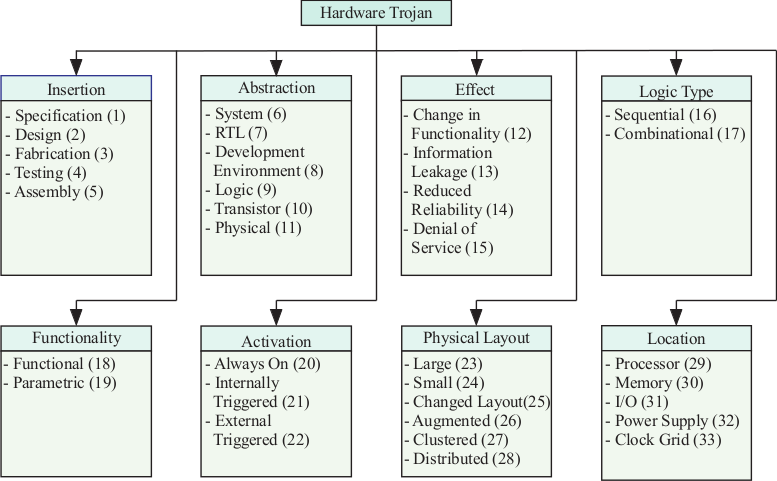
\includegraphics[width=0.7\linewidth]{../NewAutomated_V4/Figures/HW_trojan}
		\caption[Hardware Trojan Taxonomy~\cite{samerAttribute}]{Hardware Trojan Taxonomy~\cite{samerAttribute}}
		\label{fig:HW_trojan}
	\end{figure}
\end{frame}

\begin{frame}
	\frametitle{Relation Matrix}
	\begin{figure}
		\centering
		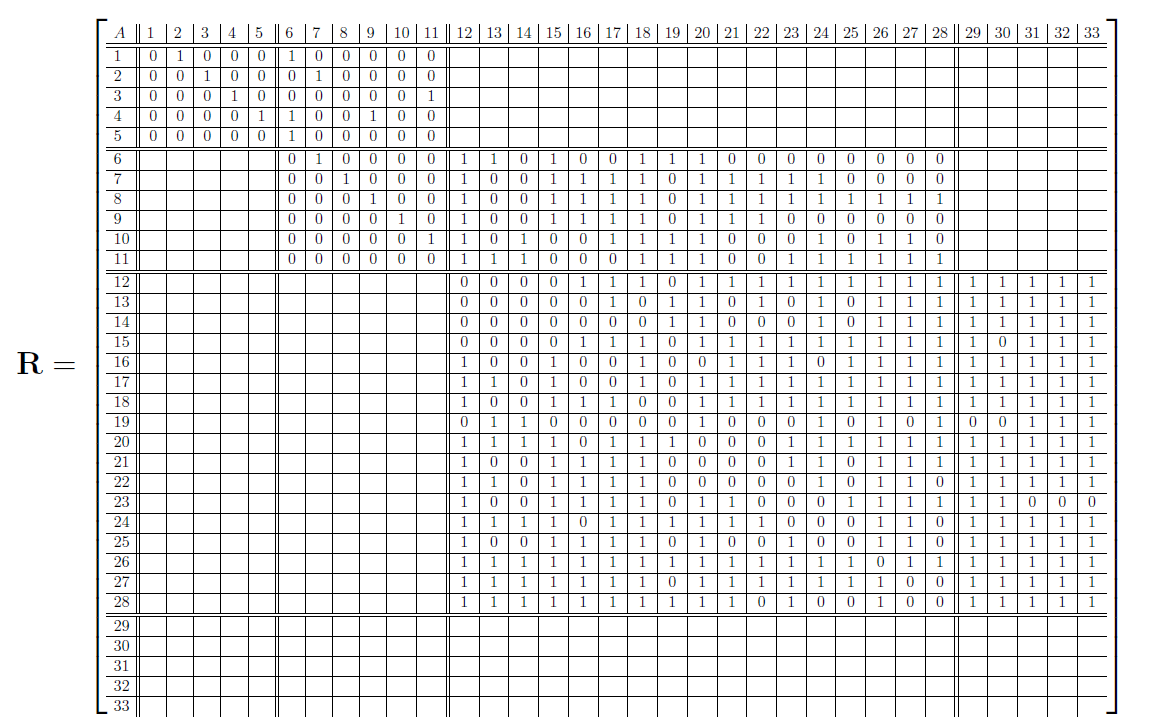
\includegraphics[width=0.9\linewidth]{figs/R}
		\caption[Relation Matrix R]{Relation Matrix R}
		\label{fig:R}
	\end{figure}
\end{frame}

%\begin{frame}
%	\frametitle{Trojan Detector: Direct Observation (Location Category)}
%	\begin{enumerate}
%		\item The \textbf{Processor} attribute pertains to the core functionality of the design logic. It can be awarded for presence of a modified Configurable Logic Block (CLB) tile or Interconnect tile.
%		\item The \textbf{Memory} attribute can be awarded for the presence of modified Block RAM  (BRAM) components.
%		\item The \textbf{Input-Output} attribute can be awarded for presence of modified Input-Output tiles.
%		\item The \textbf{Power Supply} attribute can be awarded for the presence of modified interface or configuration tiles.
%		\item The \textbf{Clock Grid} attribute can be awarded for modified clock tiles.
%	\end{enumerate}
%\end{frame}
%
%\begin{frame}
%	\frametitle{Trojan Detector: Helper Methods (Scatter Score)}
%	
%\end{frame}
\begin{frame}
	\frametitle{Trojan Detector: User-Interface}
	\begin{figure}
		\centering
		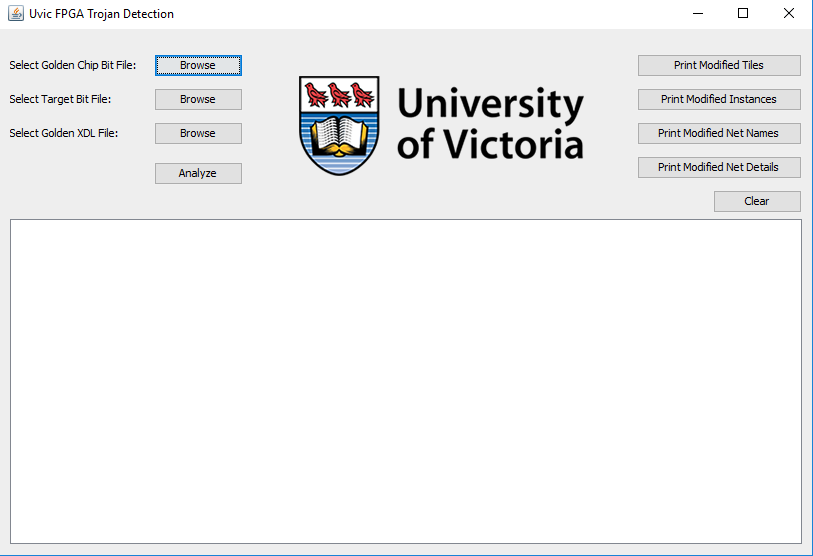
\includegraphics[width=0.7\linewidth]{figs/trojanDetectorUI}
		\caption[Hardware Trojan Detector User-Interface]{Hardware Trojan Detector User-Interface}
		\label{fig:trojanDetectorUI}
	\end{figure}
\end{frame}

\section{Hardware Trojan System (HTS)}
\begin{frame}
	\frametitle{HTS: Classification Tool}
	\begin{itemize}
		\item Allows users to pick attributes observed in their trojan using a simple user-interface.
		\item Generates a directed graph visual.
		\item Generates a severity vector rating.
		\item Allows users to save entries to the database for future use.
	\end{itemize}
\end{frame}

%\begin{frame}
%	\frametitle{HTS: Evaluation Tool}
%	\begin{itemize}
%		\item Allows users to search the database for known trojans and their corresponding severity rating.
%		\item Allows users to search the database for known detection methods.
%		\item Allows users to perform comparisons.
%	\end{itemize}
%\end{frame}

\section{Case Study}
\begin{frame}
	\frametitle{Case Study: AES-T100}
	\begin{displaycquote}{trustHubPaper}
		The Trojan leaks the secret key from a cryptographic chip running the AES algorithm through a covert channel. The channel adapts the concepts from spread spectrum communications (also known as Code-Division Multiple Access (CDMA)) to distribute the leakage of single bits over many clock cycles. The Trojan employs this method by using a pseudo-random number generator (PRNG) to create a CDMA code sequence, the PRNG initialized to a predefined value. The code sequence is then used to XOR modulate the secret information bits. The modulated sequence is forwarded to a leakage circuit (LC) to set up a covert CDMA channel in the power side-channel. The LC is realized by connecting eight identical flip-flop elements to the single output of the XOR gate to mimic a large capacitance.
	\end{displaycquote}
\end{frame}

\begin{frame}
	%\frametitle{Case Study: Detection}
	\begin{itemize}
		\item Attribute 3: Fabrication
		\item Attribute 4: Testing
		\item Attribute 5: Assembly
		\item Attribute 6: System
		\item Attribute 7: RTL
		\item Attribute 13: Information Leakage
		\item Attribute 16: Sequential
		\item Attribute 18: Functional
		\item Attribute 20: Always On
		\item Attribute 24: Large
		\item Attribute 26: Augmented
		\item Attribute 27: Distributed
		\item Attribute 29: Processor
		\item Attribute 30: Memory
		\item Attribute 31: IO
		\item Attribute 32: Power Supply
		\item Attribute 33: Clock Grid
	\end{itemize}
\end{frame}

\begin{frame}
	\frametitle{Case Study: Visualization}
	\begin{figure}
		\centering
		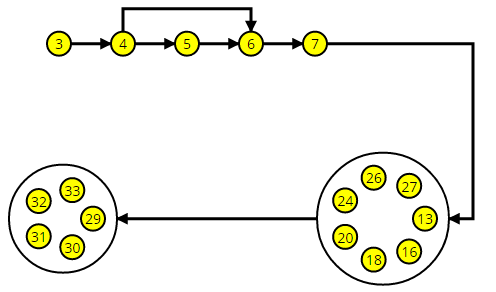
\includegraphics[width=0.7\linewidth]{../Thesis/Figures/aesVisual}
		\caption[Directed Graph of the AES-T100 Benchmark]{Directed Graph of the AES-T100 Benchmark}
		\label{fig:aesVisual}
	\end{figure}
\end{frame}
%------------------------------------------------
%\section{First Section} % Sections can be created in order to organize your presentation into discrete blocks, all sections and subsections are automatically printed in the table of contents as an overview of the talk
%%------------------------------------------------
%
%\subsection{Subsection Example} % A subsection can be created just before a set of slides with a common theme to further break down your presentation into chunks
%
%\begin{frame}
%\frametitle{Paragraphs of Text}
%Sed iaculis dapibus gravida. Morbi sed tortor erat, nec interdum arcu. Sed id lorem lectus. Quisque viverra augue id sem ornare non aliquam nibh tristique. Aenean in ligula nisl. Nulla sed tellus ipsum. Donec vestibulum ligula non lorem vulputate fermentum accumsan neque mollis.\\~\\
%
%Sed diam enim, sagittis nec condimentum sit amet, ullamcorper sit amet libero. Aliquam vel dui orci, a porta odio. Nullam id suscipit ipsum. Aenean lobortis commodo sem, ut commodo leo gravida vitae. Pellentesque vehicula ante iaculis arcu pretium rutrum eget sit amet purus. Integer ornare nulla quis neque ultrices lobortis. Vestibulum ultrices tincidunt libero, quis commodo erat ullamcorper id.
%\end{frame}
%
%%------------------------------------------------
%
%\begin{frame}
%\frametitle{Bullet Points}
%\begin{itemize}
%\item Lorem ipsum dolor sit amet, consectetur adipiscing elit
%\item Aliquam blandit faucibus nisi, sit amet dapibus enim tempus eu
%\item Nulla commodo, erat quis gravida posuere, elit lacus lobortis est, quis porttitor odio mauris at libero
%\item Nam cursus est eget velit posuere pellentesque
%\item Vestibulum faucibus velit a augue condimentum quis convallis nulla gravida
%\end{itemize}
%\end{frame}
%
%%------------------------------------------------
%
%\begin{frame}
%\frametitle{Blocks of Highlighted Text}
%\begin{block}{Block 1}
%Lorem ipsum dolor sit amet, consectetur adipiscing elit. Integer lectus nisl, ultricies in feugiat rutrum, porttitor sit amet augue. Aliquam ut tortor mauris. Sed volutpat ante purus, quis accumsan dolor.
%\end{block}
%
%\begin{block}{Block 2}
%Pellentesque sed tellus purus. Class aptent taciti sociosqu ad litora torquent per conubia nostra, per inceptos himenaeos. Vestibulum quis magna at risus dictum tempor eu vitae velit.
%\end{block}
%
%\begin{block}{Block 3}
%Suspendisse tincidunt sagittis gravida. Curabitur condimentum, enim sed venenatis rutrum, ipsum neque consectetur orci, sed blandit justo nisi ac lacus.
%\end{block}
%\end{frame}
%
%%------------------------------------------------
%
%\begin{frame}
%\frametitle{Multiple Columns}
%\begin{columns}[c] % The "c" option specifies centered vertical alignment while the "t" option is used for top vertical alignment
%
%\column{.45\textwidth} % Left column and width
%\textbf{Heading}
%\begin{enumerate}
%\item Statement
%\item Explanation
%\item Example
%\end{enumerate}
%
%\column{.5\textwidth} % Right column and width
%Lorem ipsum dolor sit amet, consectetur adipiscing elit. Integer lectus nisl, ultricies in feugiat rutrum, porttitor sit amet augue. Aliquam ut tortor mauris. Sed volutpat ante purus, quis accumsan dolor.
%
%\end{columns}
%\end{frame}
%
%%------------------------------------------------
%\section{Second Section}
%%------------------------------------------------
%
%\begin{frame}
%\frametitle{Table}
%\begin{table}
%\begin{tabular}{l l l}
%\toprule
%\textbf{Treatments} & \textbf{Response 1} & \textbf{Response 2}\\
%\midrule
%Treatment 1 & 0.0003262 & 0.562 \\
%Treatment 2 & 0.0015681 & 0.910 \\
%Treatment 3 & 0.0009271 & 0.296 \\
%\bottomrule
%\end{tabular}
%\caption{Table caption}
%\end{table}
%\end{frame}
%
%%------------------------------------------------
%
%\begin{frame}
%\frametitle{Theorem}
%\begin{theorem}[Mass--energy equivalence]
%$E = mc^2$
%\end{theorem}
%\end{frame}
%
%%------------------------------------------------
%
%\begin{frame}[fragile] % Need to use the fragile option when verbatim is used in the slide
%\frametitle{Verbatim}
%\begin{example}[Theorem Slide Code]
%\begin{verbatim}
%\begin{frame}
%\frametitle{Theorem}
%\begin{theorem}[Mass--energy equivalence]
%$E = mc^2$
%\end{theorem}
%\end{frame}\end{verbatim}
%\end{example}
%\end{frame}
%
%%------------------------------------------------
%
%\begin{frame}
%\frametitle{Figure}
%Uncomment the code on this slide to include your own image from the same directory as the template .TeX file.
%%\begin{figure}
%%\includegraphics[width=0.8\linewidth]{test}
%%\end{figure}
%\end{frame}
%
%%------------------------------------------------
%
%\begin{frame}[fragile] % Need to use the fragile option when verbatim is used in the slide
%\frametitle{Citation}
%An example of the \verb|\cite| command to cite within the presentation:\\~
%
%This statement requires citation \cite{p1}.
%\end{frame}
%
%%------------------------------------------------
%
\begin{frame}
\frametitle{References}
\footnotesize{
\begin{thebibliography}{99} % Beamer does not support BibTeX so references must be inserted manually as below
\bibitem[Moein, 2016]{samerAttribute} S.~Moein and T.~A. Gulliver and F.~Gebali and A.~Alkandari (2016)
\newblock A New Characterization of Hardware Trojans
\newblock \emph{IEEE Access} v4, 2721 -- 2731.

\bibitem[Zhang, 2016]{fpgaTrojanSurvey2014} J.~Zhang and G.~Qu (2014)
\newblock A survey on security and trust of FPGA-based systems
\newblock \emph{Field-Programmable Technology} 147 -- 152.

\bibitem[Li, 2015]{hardwareTrojanSurvey2015} H.~Li and Q.~Liu and J.~Zhang and Y.~Lyu (2015)
\newblock A Survey of Hardware Trojan Detection, Diagnosis and Prevention
\newblock \emph{2015 14th International Conference on Computer-Aided Design and Computer Graphics (CAD/Graphics)} 173 -- 180.

\bibitem[Salmani, 2015]{trustHubPaper} H.~Salmani and M.~Tehranipoor and R.~Karri (2013)
\newblock On design vulnerability analysis and trust benchmarks development
\newblock \emph{2013 IEEE 31st International Conference on Computer Design (ICCD)} 471 -- 474.
\end{thebibliography}
}
\end{frame}
%
%%------------------------------------------------
%
\begin{frame}
\Huge{\centerline{The End}}
\end{frame}

%----------------------------------------------------------------------------------------

\end{document} 